\documentclass{article}
\usepackage{amsmath}
\usepackage{graphicx}
\usepackage{mathtools}
\usepackage{fullpage}
\usepackage{float}

\begin{document}
\title{6.867: Homework 1}
\author{Andres Hasfura and Kathryn Evans}
\maketitle
\section{Gradient Descent}
Gradient descent works by updating an initial guess by taking a step opposite the direction of the gradient at that initial guess. Moving opposite the gradient helps  to effectively move "downhill" in terms of the function value.  The formulation of the gradient descent method is as follows
\begin{equation}
x(\tau+1) = x(\tau) - \alpha \nabla F(x(\tau))
\end{equation}

Where $ x(\tau)$ is the current guess, with $\tau$ being the current iteration, $\alpha$ is the step size and $F(x)$ is the function which will be evaluated. This method is carried out until there is convergence, which is checked by looking at the norm of successive guesses and seeing if it is less than the required tolerance, $\epsilon$,   



\begin{equation} 
\left \lVert x(\tau+1)-x(\tau) \right \rVert \leq \epsilon
\end{equation}

This is implemented in the code, $grad\_descent.m$ which takes arguments, $x_i, \alpha, \epsilon, f,$ and $df$ where $f$, and $df$ are function handles and returns $x_{min}, f(x_{min})$



\subsection*{ Gradient Descent Benchmarking}


We implemented this code on a few different functions, first simply a 1-D quadratic bowl, then on a N-D quadratic bowl 



Implementing the gradient descent code on a sine wave, which has multiple minima,  allowed us to investigate better the effects of input parameters on the declared minima. The figures below show the effect of changing the initial guess and the tolerance. 
\begin{figure}[H]
\begin{minipage}{.3\textwidth}
\center
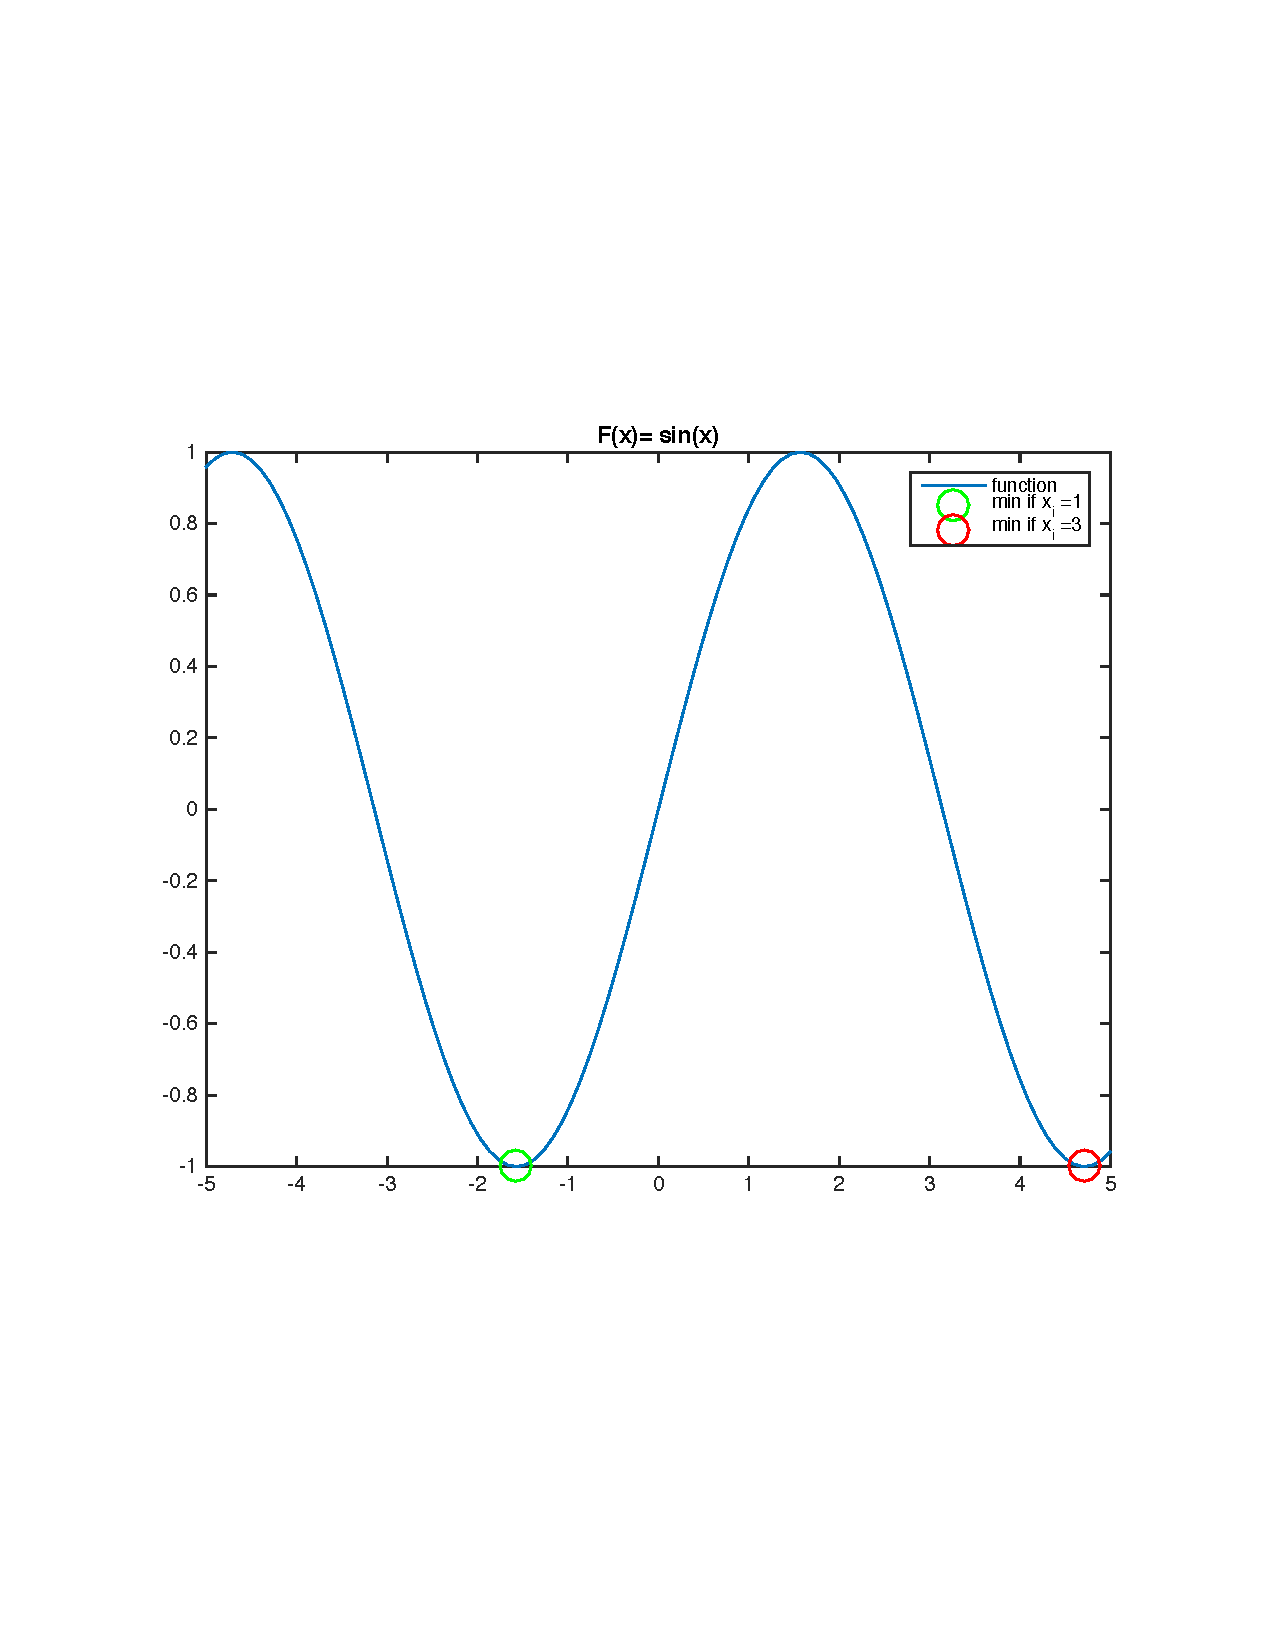
\includegraphics[scale=.25]{1Dsin.pdf}
	
\end{minipage}
\begin{minipage}{.3\textwidth}
\center
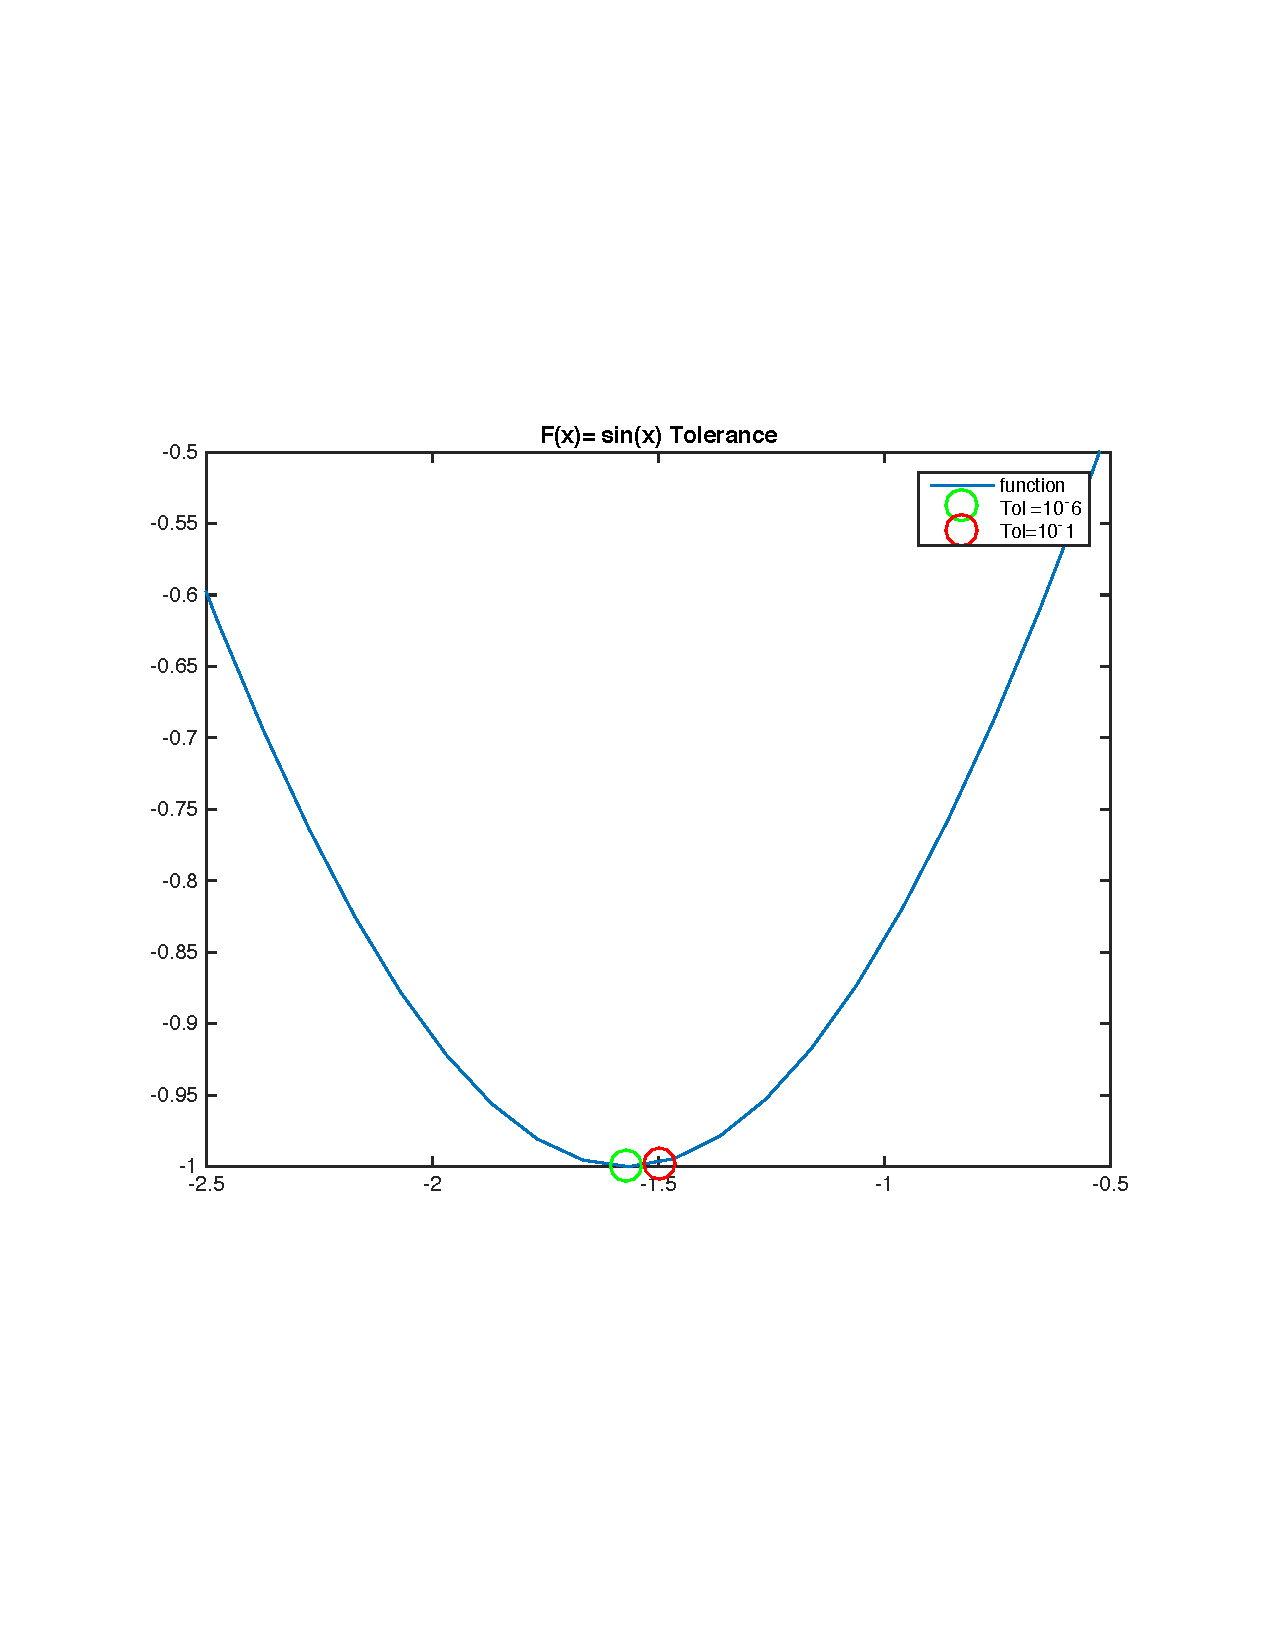
\includegraphics[scale=.25]{1DsinHighTol.pdf}
	
\end{minipage}
\begin{minipage}{.3\textwidth}
\center
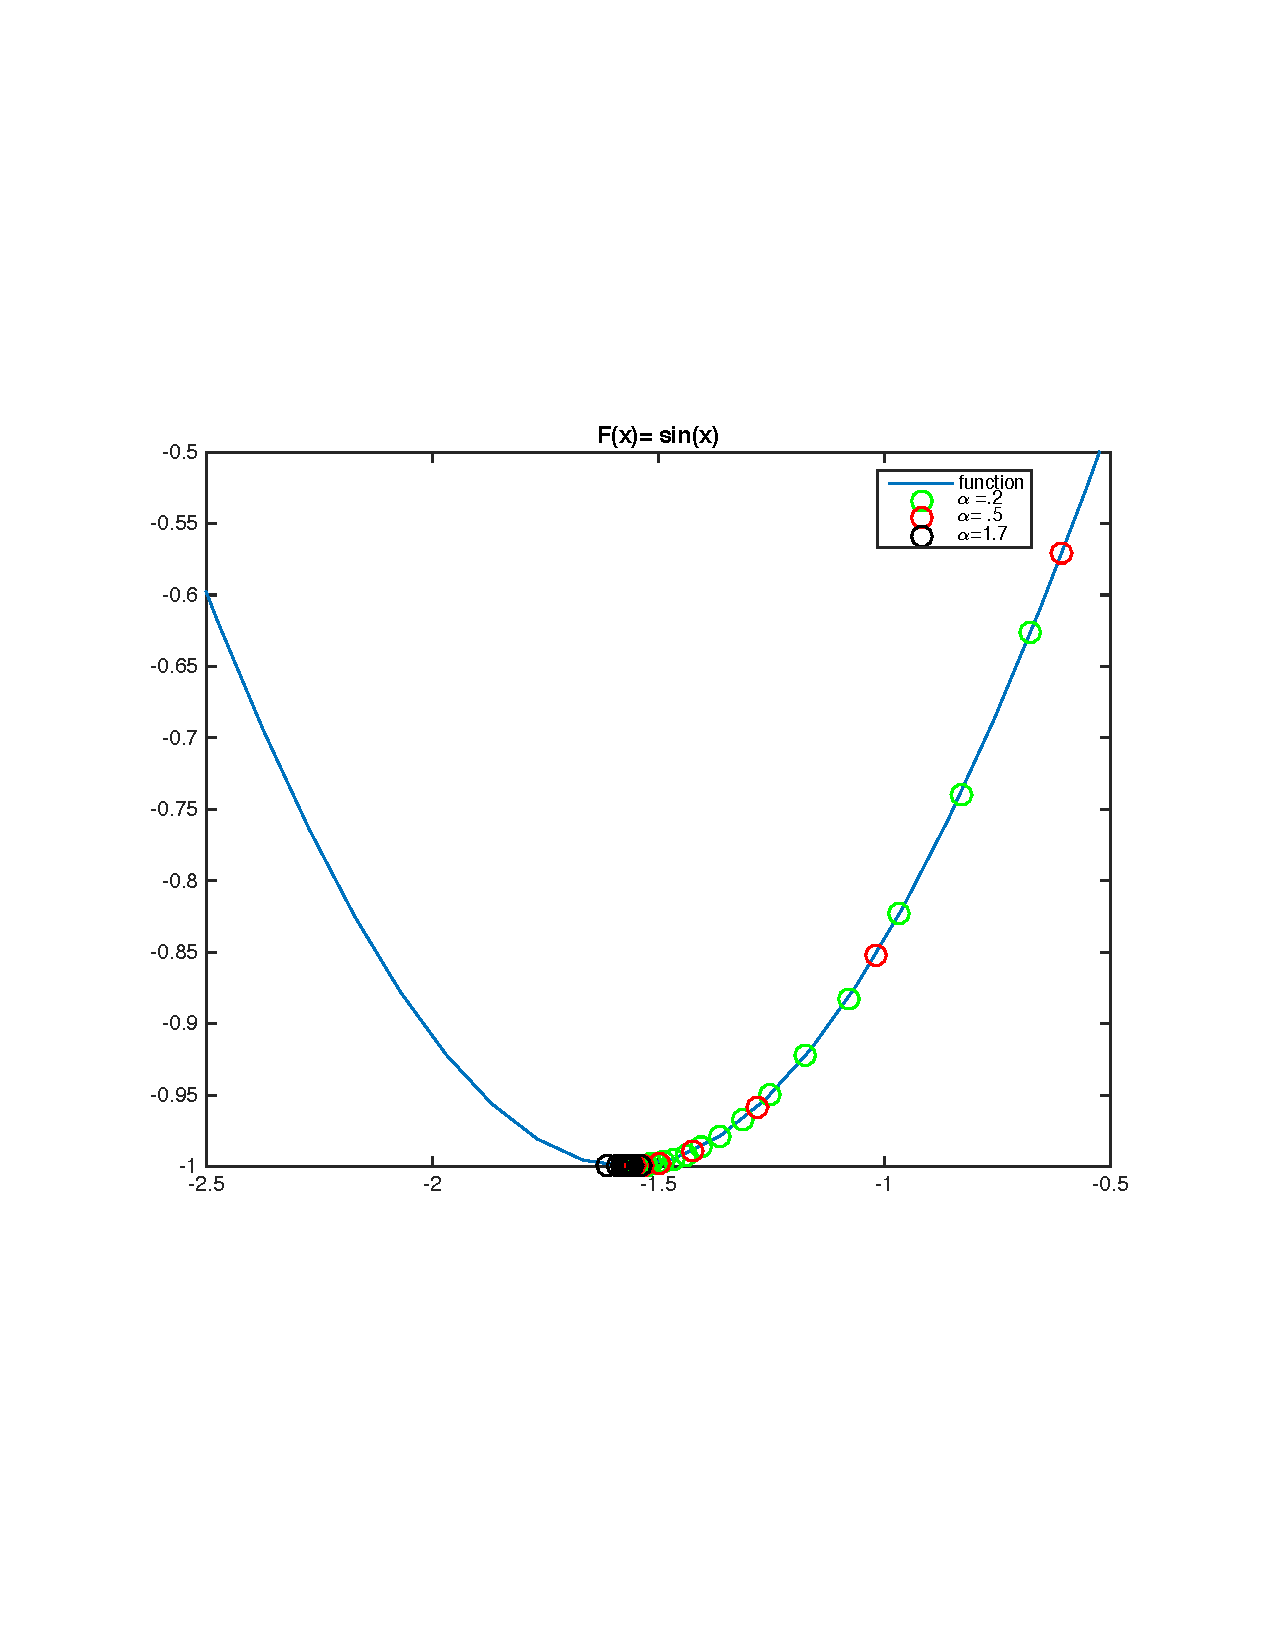
\includegraphics[scale=.25]{1DsinStepSize.pdf}
\end{minipage}
\caption{ Effect of changing input parameters. a) shows the effect of different initial guess leads to a different minimum. b) Setting tolerances too large does not capture true minimum. c) Setting step size too small increases number of iterations. Setting it too large also increases number of iterations by overshooting the minimum}
\end{figure}

By changing the initial guess at points where the slopes head towards different minima of course changes the output of the gradient descent process. If the tolerance is too high, the solver converges too quickly and does not find the true minima.  Changing the step size caused an increase in computation time because if it is excessively small, the number of steps increases dramatically and it if it is too large the solver can overshoot the minima. 
 
\end{document}